\clearpage
\section{Diseño del sistema}\label{sec:sistema}

\begin{figure}[H]
\centering
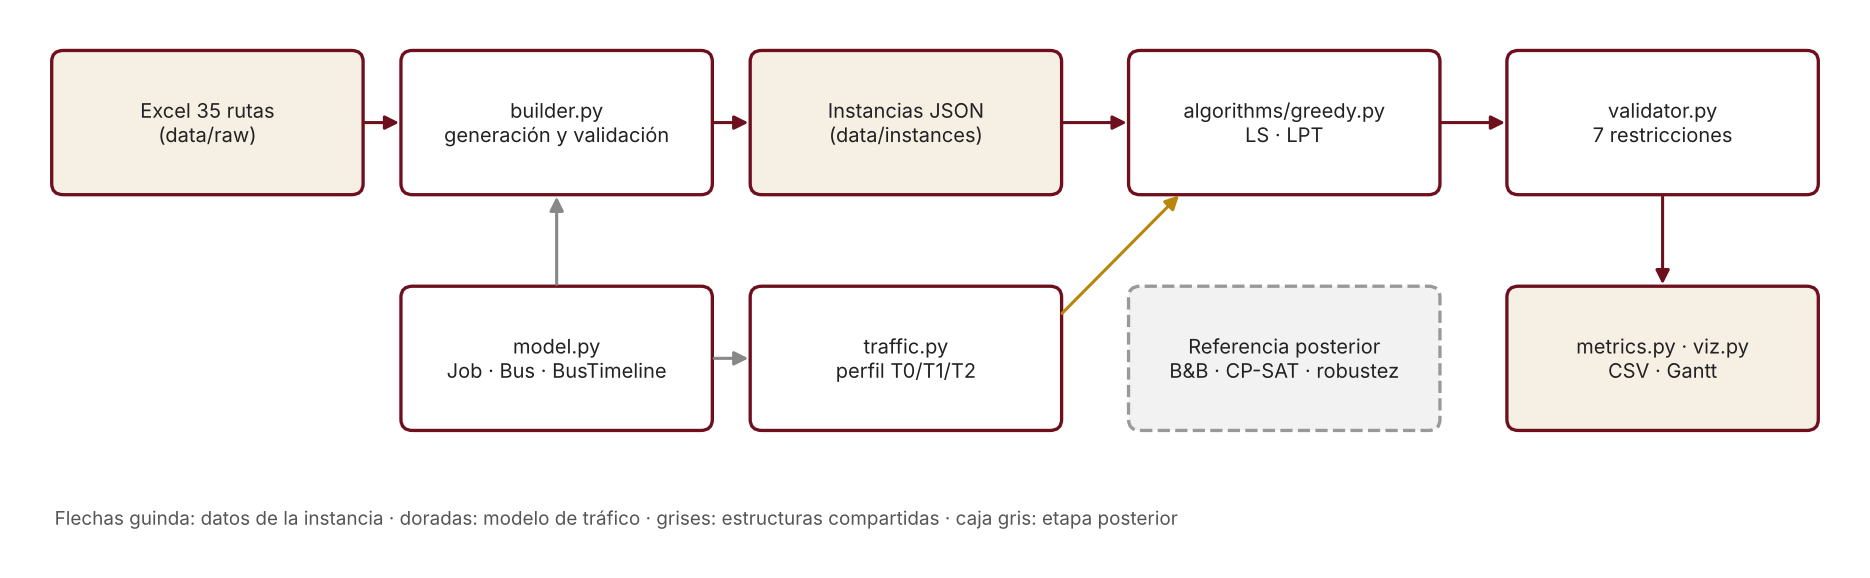
\includegraphics[width=\textwidth]{figuras/fig_arquitectura.png}
\caption{Módulos del sistema y flujo de información (la caja punteada corresponde a etapas posteriores).}\label{fig:arquitectura}
\end{figure}

El flujo es general para todas las rutas: datos de la ruta $\to$ parámetros del modelo $\to$ generación de vueltas $\to$ ventanas $\to$ tráfico $\to$ LS/LPT $\to$ validación $\to$ resultados. El Excel del proyecto se transforma en instancias JSON validadas; cada instancia se resuelve con el algoritmo y el perfil de tráfico elegidos, el validador revisa la solución y se generan métricas, archivos CSV y diagramas de Gantt.

\begin{table}[H]
\centering\small
\caption{Módulos del paquete \texttt{bus\_sched}.}
\begin{tabularx}{\textwidth}{L{5.4cm}Y}
\toprule
Módulo & Responsabilidad \\
\midrule
\texttt{traffic.py} & Perfiles T0/T1/T2 y cálculo de $p_j(s)$. \\
\texttt{model.py} & Vueltas, buses, instancia, línea de tiempo por bus (\texttt{BusTimeline}) y solución (\texttt{Schedule}). \\
\texttt{builder.py} & Lectura del Excel, regla general de generación de vueltas y ventanas, validación de datos, instancia del ejemplo manual. \\
\texttt{algorithms/greedy.py} & List Scheduling y LPT. \\
\texttt{validator.py} & Verificación independiente de todas las restricciones. \\
\texttt{metrics.py} & Vueltas atendidas, $\Lmax$, cota inferior y brecha, desbalance, utilización, saturación $\rho$. \\
\texttt{viz.py}, \texttt{cli.py} & Diagramas de Gantt e interfaz de línea de comandos (\texttt{python -m bus\_sched}). \\
\texttt{algorithms/bnb.py}, \texttt{algorithms/cpsat.py}, \texttt{simulation.py} & Prototipos de los mecanismos de referencia y de robustez previstos para etapas posteriores. \\
\bottomrule
\end{tabularx}
\end{table}

\textbf{Formatos.} Las instancias se guardan en JSON, una por ruta, con horas en formato HH:MM y duraciones en minutos:
\begin{lstlisting}
{"route": "RTI-01", "company": "E.T. SAYLLA S.A.", "day_start": "06:00", "day_end": "22:00",
 "buses": [{"id": "RTI-01-B1", "lunch_r": "10:30", "lunch_d": "11:30", "lunch_min": 120}, ...],
 "jobs":  [{"id": "RTI-01-J001", "base_min": 148.8, "r": "06:00", "d": "06:15", "nominal": "06:00"}, ...]}
\end{lstlisting}
Los perfiles de tráfico usan JSON con franjas (inicio, fin, factor). La salida de cada ejecución es un CSV con una fila por vuelta: ruta, vuelta, bus, ventana, salida, llegada, duración con tráfico y duración base; las vueltas no atendidas llevan \texttt{bus = NO\_ASIGNADO}. Todas las rutas de archivo son relativas al repositorio.
